\documentclass[prodmode,acmtoms]{acmsmall}
%  

% Package to generate and customize Algorithm as per ACM style
\usepackage[ruled]{algorithm2e}
\renewcommand{\algorithmcfname}{ALGORITHM}
\SetAlFnt{\small}
\SetAlCapFnt{\small}
\SetAlCapNameFnt{\small}
\SetAlCapHSkip{0pt}
\IncMargin{-\parindent}

% Metadata Information
\acmVolume{0}
\acmNumber{0}
\acmArticle{00}
\acmYear{0000}
\acmMonth{0}

%
%%% User-requested packages placed after this line %%%%%%%%%%%%%%%%%%%%%%%%%%%%
\usepackage{amsfonts,amssymb,amsmath}
\usepackage{booktabs,dcolumn}
\usepackage[T1]{fontenc}
\usepackage{mathtools}
\usepackage{enumerate,graphicx}
\usepackage{subfig}
\usepackage{multirow}
\usepackage{listings}

% \usepackage[center]{subfigure}
\numberwithin{equation}{section}
\usepackage{braket}                             %Provides \Set for typing sets
\usepackage{float}
\usepackage{subfig}


%%% User's macros placed after this line %%%%%%%%%%%%%%%%%%%%%%%%%%%%%%%%%%%%%%
%\IfFileExists{dsfont.sty}%
%\usepackage{dsfont}
\newcommand{\R}{\mathbb{R}}
\newcommand{\N}{\mathbb{N}}
\renewcommand{\phi}{\varphi}
\renewcommand{\epsilon}{\varepsilon}

\newcommand{\todo}[1]{\textbf{\textsc{\textcolor{black}{TODO: #1}}}}

%
\begin{document}
\markboth{C. Goll, T. Wick, and W. Wollner}{DOpElib: A Goal Oriented Software Library}

\title{DOpElib: A Goal Oriented Software Library for Computing PDEs and Optimization Problems}

\author{CHRISTIAN GOLL
\affil{University of Heidelberg}
THOMAS WICK
\affil{The University of Texas at Austin}
WINNIFRIED WOLLNER
\affil{University of Hamburg}}

%%%%%%%%%%%%%%%%%%%%%%%%%%%%%%%%%%%%%%%%%%%

\begin{abstract}
In this article, we describe the software library 
\textit{Deal.II Optimization Environment} (DOpElib).
The main feature of DOpElib is that it provides a unified interface to high level algorithms 
such as time stepping methods, nonlinear solvers and optimization routines. This structure ensures 
that first of all the user is required to write those sections of code that are specific to 
the considered problem. Second, the exchange of parts of the used routines is possible 
with the need for just a few lines of code to change.
The article illustrates performance and features 
of the software package by four numerical tests. 
\end{abstract}

%\category{C.2.2}{Computer-Communication Networks}{Network Protocols}

%\terms{Design, Algorithms, Performance}

%\keywords{Wireless sensor networks, media access control,
%multi-channel, radio interference, time synchronization}

%\acmformat{Zhou, G., Wu, Y., Yan, T., He, T., Huang, C., Stankovic,
%J. A., and Abdelzaher, T. F.  2010. A multifrequency MAC specially
%designed for  wireless sensor network applications.}

\begin{bottomstuff}
Author's adresses: C. Goll, Institut f\"ur Angewandte Mathematik,
Universit\"at Heidelberg;
T. Wick, The Institute for Computational Engineering and Sciences;
W. Wollner, Fachbereich Mathematik, Universit\"at Hamburg.
\end{bottomstuff}
                      

\maketitle
%%%%%%%%%%%%%%%%%%%%%%%%%%%%%%%%%%%%%%%%%%%


%%%%%%%%%%%%%%%%%%%%%%%%%%%%%%%%%%%%%%%%%%%
\section{Introduction}
\label{introduction}
The \textit{Deal Optimization Environment} (DOpElib) 
provides a software toolkit to solve forward PDE
problems as well as optimal control problems constrained by a PDE. 
Its main feature is to give a unified interface to high level algorithms such as 
time stepping methods, nonlinear solvers and optimization routines. 
We aim that the user should only need to write those parts
of the code that are problem dependent while all invariant parts of the algorithms
should be reusable without any need for further coding.
In particular, the user should be able to switch between various different 
algorithms without the need to rewrite the problem dependent code, though he or she will
have to replace the algorithm object with an other one. 

The
solution of a broad variety of PDE is possible in other software
libraries (like in deal.II \cite{deal}, dune \cite{dune} , 
or commercial solvers like Ansys \cite{ansys}) 
as well, but
DOpE concentrates on a unified approach for both linear and nonlinear
problems by interpreting every PDE problem as nonlinear and applying a
Newton method to solve it. While deal.II leaves much of the work and many
decisions to the user, DOpE intends to be user-optimized by delivering
prefabricated tools which require from the user only adjustments connected
to his specific problem. The solution of optimal control problems with PDE
constraints is an innovation in the DOpE framework.
The focus is on the numerical solution of both stationary and nonstationary
problems which come from different application fields, like elasticity and
plasticity, fluid dynamics, and fluid-structure interactions.

The DOpElib project is 
based on the \textit{deal.II} \cite{deal} finite element library which has been developed
 initially by W. Bangerth, R. Hartmann, and G. Kanschat \cite{deal}.
The authors acknowledge their past experience as well as discussions with 
the authors of the libraries 
Gascoigne/RoDoBo project, which was initiated by 
Roland Becker, Dominik Meidner,  and Boris Vexler \cite{rodobo}. 
From which some of the ideas to modularize the algorithms have arisen.

%%%%%%%%%%%%%%%%%%%%%%%%%%%%%%%%%%%%%%%%%%%%%%%%%%%
%The aim of DOpE is to provide a software toolkit to solve forward PDE
%problems as well as optimal control problems constrained by PDE. The
%solution of a broad variety of PDE is possible in deal.II as well, but
%DOpE concentrates on a unified approach for both linear and nonlinear
%problems by interpreting every PDE problem as nonlinear and applying a
%Newton method to solve it. While deal.II leaves much of the work and many
%decisions to the user, DOpE intends to be user-optimized by delivering
%prefabricated tools which require from the user only adjustments connected
%to his specific problem. The solution of optimal control problems with PDE
%constraints is an innovation in the DOpE framework.
%The focus is on the numerical solution of both stationary and nonstationary
%problems which come from different application fields, like elasticity and
%plasticity, fluid dynamics, and fluid-structure interactions.
%

At the present stage the following key features are supported by the library
\begin{itemize}
\item Solution of stationary and nonstationary PDEs in 1d, 2d, and 3d.
\item Various time stepping schemes (based on finite differences), 
  such as forward Euler, backward Euler,
  Crank-Nicolson, shifted Crank-Nicolson, and Fractional-Step-$\Theta$ scheme.
\item All finite elements of from deal.II including hp-support.
\item Several examples showing the solution of several PDEs including
   Poisson, Navier-Stokes, Plasticity and fluid-structure interaction problems. 
\item Self written line search and trust region newton algorithms for the 
   solution of optimization problems with PDEs \cite{NoWr00}
\item Interface to SNOPT for the solution of optimization problems with PDEs and
  additional other constraints.
\item Several examples showing how to solve various kinds of optimization problems
  involving stationary PDE constraints.
\item Goal-oriented mesh adaptation with the dual-weighted residual method.
\item Different spatial triangulations for control and state variables.
\end{itemize}

The article is organized as follows. In Section
\ref{detailed_description} 
 
%The rest of this document is structured as follows: We start with an introduction in
%Chapter~\ref{chap:intro} where you will learn what is needed to run {\tt DOpElib}. 
%Further you will learn what problems we can solve and how all the different classes 
%work together for this purpose. This should help you figure out what the different classes
%do if you are in need of writing your own algorithm.
%
%Then assuming that you can work to your satisfaction with the algorithms already implemented
%we will show you how to create your own running example in Chapter~\ref{chap:howtoex}.
%This will be followed by a detailed description of all examples already shipped with 
%the library. You can find the examples for the solution of PDEs in Chapter~\ref{PDE}
%and those for the solution of optimization problems with PDEs in Chapter~\ref{OPT}.
%
%These notes conclude with a section that explains how we do automated testing of the 
%implementation in Chapter~\ref{chap:test}. This chapter will be of interest only if you 
%are trying to implement some new features to the library so that you can check that 
%the new code did not break anything.
%



%%%%%%%%%%%%%%%%%%%%%%%%%%%%%%%%%%%%%%%%%%%
\section{Detailed Description of the Main Features}
\label{detailed_description}
%\todo{Aus der Sicht des Users anhand eines konkreten Beispiels beschreiben}
%\todo{Einfaches Beispiel nehmen}
%\todo{erwaehnen, dass wir alles immer nicht-linear betrachten}
%\todo{Aussehen eines typischen PDE und Opt loop und deren Gemeinsamkeiten
%erklaeren. Vielleicht mir Pseudocode}
This library is designed to allow easy implementation and numerical solutions 
of problems involving partial differential equations (PDEs). 
\subsection{Solving of PDEs}
\subsubsection{Stationary problems}
The easiest case 
is that of a PDE in weak form to find some $u$
\[
a(u)(\phi) = 0 \quad \forall \phi \in V,
\]
with some appropriate space $V$. As example, we take 
the Laplace problem in weak form:
\[
a(u)(\phi) = (\nabla u, \nabla \phi) \quad \forall \phi \in V.
\]
To solve the problem, we need a configuration (a mesh), eventually 
a diffusion parameter, a finite element, a quadrature rule,
a linear solver (here the CG solver), and some output such as
a graphical solution and eventually some measurement functional.
Each of those routines are written in the \texttt{main.cc} file. 
We start by including necessary files both the DOpElib library and
the deal.II software:
\begin{lstlisting}
  #include "pdeproblemcontainer.h" etc. ...
\end{lstlisting}
In the \texttt{main} function, the following steps need to be done. First, 
the parameter reader for runtime parameters is initialized:
\begin{lstlisting}
  ParameterReader pr;
  SSolver::declare_params(pr);
  DOpEOutputHandler<VECTOR>::declare_params(pr);
  pr.read_parameters(paramfile);
\end{lstlisting}
A linear finite element in two dimensions and two components is 
initialized:
\begin{lstlisting}
  FESystem<2> state_fe(FE_Q<2>(1), 2);
\end{lstlisting}
and a quadrature rule of order three is used to approximate the 
integrals:
\begin{lstlisting}
  QGauss<2> quadrature_formula(3);
\end{lstlisting}
Then, the \texttt{LocalPDE} object comes into play. This is an quite 
important feature of DOpElib because it allows for easy implementation 
of the variational formulation. Specific explication is given below because
the implementation is seperated in \texttt{localpde.h}.
Afterwards, a \texttt{LocalPointFunctional} is declared. As for the PDE, the 
implementation is done in another file, namely \texttt{localfunctional.h}.

Generically, each problem in DOpElib is considered to be time-dependent and nonlinear because
these are the 'real' world problems. Therefore, (even for the linear and stationary Laplace equation),
we have to declare a (pseudo) time:
\begin{lstlisting}
  std::vector<double> times(1, 0.);
\end{lstlisting}
Then, the spatial mesh (here the unit square) is created and three-times globally-refined:
\begin{lstlisting}
  GridGenerator::hyper_cube(triangulation, 0, 1);
  triangulation.refine_global(3);
\end{lstlisting}
A major component which organizes the whole solution process (independent from 
the problem!) is the 
\begin{lstlisting}
  MethodOfLines_StateSpaceTimeHandler<FE, DOFHANDLER, 
    SPARSITYPATTERN, VECTOR, 2> DOFH(triangulation, state_fe);
\end{lstlisting}
This method handles all dofs in space and time and different versions exist
for forward as well as optimization problems.

Afterwards, the problem (here the Laplace PDE) is given to the \texttt{DOFH} via
\begin{lstlisting}
  OP P(LPDE, DOFH);
\end{lstlisting}
It remains to declare boundary conditions for the problem under consideration. 
Let's simply take zero Dirichlet conditions on the boundary:
\begin{lstlisting}
  std::vector<bool> comp_mask(2);

  comp_mask[0] = true;
  comp_mask[1] = true;

  DOpEWrapper::ZeroFunction<2> zf(2);
  SimpleDirichletData<VECTOR, 2> DD1(zf);

  P.SetDirichletBoundaryColors(0, comp_mask, &DD1);
\end{lstlisting}
Next, the solver for the linear equations needs to be specified:
\begin{lstlisting}
  SSolver solver(&P, "fullmem", pr, idc);
\end{lstlisting}
Finally, the ouput handler is initialized via
\begin{lstlisting}
  P.RegisterOutputHandler(&out);
  solver.RegisterOutputHandler(&out);
\end{lstlisting}
Finally, the programm is started with:
\begin{lstlisting}
  solver.ReInit();
  out.ReInit();
  out.Write(outp, 1, 1, 1);
  solver.ComputeReducedFunctionals();
\end{lstlisting}
After explaining the basic compononents that are necessary for all  
(linear and stationary) partial differential equations, we shall give 
an overview to the implementation of the specific form of the PDE. 
This step is done in the \texttt{localpde.h} file. As already explained,
each PDE is treatet in a nonlinear manner such that for solving 
the Laplace problem the following nonlinear step is necessary to recapitulate:
Find $\delta u\in V$:
\[
(\nabla \delta u, \nabla \phi) = -(\nabla u, \nabla \phi) 
\]
and $u^{n+1} = u^n + \delta u$ for $n=1,2,3,ldots$.
Therefore, the implementation reads for the right hand side:
\begin{lstlisting}
   void CellEquation(...)
    {
      // implement (\nabla u, \nabla \phi) 
    }
\end{lstlisting}
Specifically, the inner loops reads
\begin{lstlisting}
   for (all quadrature points per cell q)
      {
        Tensor<2, 2> ugrads; // solution vector
 
	for (all dofs per cell i)
        {
	  const Tensor<2, 2> phi_i_grads_u; // test function

          local_cell_vector(i) += scale * 
            scalar_product(ugrads, phi_i_grads_u) *
	    state_fe_values.JxW(q_point);
        }
      }
\end{lstlisting}
For the left hand side, we need to implement the Jacobian matrix:
\begin{lstlisting}
   void CellMatrix(...)
    {
      // implement  (\nabla \delta u, \nabla \phi)
    }
\end{lstlisting}
Specifically,
\begin{lstlisting}
      for (all quadrature points per cell q)      
        for (all dofs per cell i)    
          for (all dofs per cell j)
          {
            local_entry_matrix(i, j) += 
              scalar_product(phi_grads_u[j], phi_grads_u[i]) * 
              state_fe_values.JxW(q_point);
          }
\end{lstlisting}
The integration of the equation for each DoF and each quadrature point on each
cell is then done 
in the \texttt{templates/integrator.h} function. 


The target functional 
is now implemented in \texttt{functional.h} and 
treats a point evaluation:
\begin{lstlisting}
  double PointValue(...)
   {
    Point<2> p1(0.5, 0.5);
    Vector<double> tmp_vector(2);
    // more stuff is necessary here
    VectorTools::point_value (...);
    double x = tmp_vector(0);

    return x;
   }
\end{lstlisting}




\subsubsection{Nonstationary problems}
In this section, we focus on the extension to 
the numerical solution of nonstationary processes. 
As example, we consider the heat equation:
Find $u$:
\[
\partial_t u - \Delta u = 0
\]
and in weak formulation:
Find $u$:
\[
a(u)(\phi) = 0 \quad \forall \phi \in V,
\]
with some appropriate space $V$ and 
\[
a(u)(\phi) = (\partial_t u, \phi) + (\nabla u, \nabla \phi) \quad \forall \phi \in V.
\]
Temporal discretization using the One-step-$\theta$ scheme reads:
Given the old timestep solution $u^n$, find $u^{n+1}$:
\[
\frac{(u^{n+1} - u^{n}, \phi)}{k} + \theta (\nabla u^{n+1}, \nabla \phi)
+ (1 - \theta) (\nabla u^{n}, \nabla \phi) = 0,
\]
Reordering in new and old terms and multiplication by the time step size $k$:
\[
(u^{n+1},\phi) + k \theta (\nabla u^{n+1}, \nabla \phi)
= (u^n, \phi) - (1 - \theta) (\nabla u^{n}, \nabla \phi).
\]
In DOpElib, different time stepping schemes can be found 
in the folder \texttt{DOpEsrc/tsschemes}.

Because the \texttt{main} file 
is basically the same as for stationary problems
which is one major goal of the software library,
we only focus on the implementation of the PDE in the 
\texttt{localpde.h} file. Here, the stationary part, i.e.,
the diffusion is implemented as before. The only thing we add 
is the time-depdendent part $\partial_t u$:

\begin{lstlisting}
  void CellTimeEquation(...)
   {
     // implement (u^{n+1},\phi) 
   }
\end{lstlisting}
and it is done in a straight-forward way:
\begin{lstlisting}
  for (all quadrature points per cell q)
   {
     Tensor<1,2> u = ...;

     for (all dofs per cell i)
      {
        const Tensor<1,2> phi_i_u = ...;

        local_cell_vector(i) +=  
          scale * (u * phi_i_u) * 
          state_fe_values.JxW(q_point);
      }
   }
\end{lstlisting}
Here, the advantage is that DOpElib orders the terms in the timestepping
problems
such that only $(u^{n+1},\phi)$ must be implemented. However, if someone 
needs explicit input of the old timestep term, then he can use 
\begin{lstlisting}
  void CellTimeEquationExplicit (...)
   {
     // implement (u^{n+1},\phi) and (u^n,\phi)  
   }
\end{lstlisting}
For instance, this explicit term is used for fluid-structure interaction in
which
the old timestep term needs explicit modification.   





\subsection{Solving of optimization problems}
Upgrading the framework for solving optimization problems
is described in this section. A prototypical problem reads:
\begin{align*}
\min\;&J(q,u) \\
  &\text{s.t.}\; a(q,u)(\phi) = 0 \quad \forall \phi\in V,\\
  &a \le q \le b,\\
  &g(q,u) \le 0,  
\end{align*}
where $u$ is a FE-function and $q$ can either be a FE-function or some 
fixed number of parameters, $a$ and $b$ are constraint bounds for the control $q$,
and $g(\cdot)$ is some state constraint.
As before, the main part is done in the \texttt{main} function there is no
great difference to the previous explications. However, 
since we utilize gradient-based optimization routines \cite{...},
all derivatives must be implemented. All this information
must given to the \texttt{localpde.h} file. Herein, one has to 
implement the adjoint, tangent and adjoint Hession equations. 
The algorithmic parts are described in the literature \cite{BeMeVe06}.

Concretely, let us focus on the Laplace equation and 
the following optimization problem (taken from 
Example 2) in \texttt{Examples/OPT/StatPDE}:
\begin{align*}
\min_{(q,u)\in \mathbb R^3 \times H_0^1(\Omega; \mathbb R^2)} J(q,u) &=
\frac{1}{2} \sum_{i=0}^2 |(u-\overline u)(x_i)|^2 + \frac{\alpha}{2}\|q\|^2\\
\text{s.t.} (\nabla u,\nabla \phi) &= (f(q),\phi)\;\;\forall\,\phi \in H^1_0(\Omega; \mathbb R^2)
\end{align*}
on the domain $\Omega = [0,1]^2$, with
\begin{itemize}
\item the observation points
\begin{align*}
x_0 = (0.5, 0.5), \quad x_1 = (0.5, 0.25),\quad x_2 = (0.25, 0.25),
\end{align*}
\item the regularization parameter $\alpha = 0$, 
\item the right hand side
\begin{align*}
 f(q) &= q_0 \left(\begin{matrix}2\pi^2  \sin( \pi x) \sin(\pi y)\\0 \end{matrix}\right)\\
      &+ q_1 \left(\begin{matrix}5\pi^2  \sin( \pi x) \sin(2\pi y)\\0 \end{matrix}\right)\\
      &+ q_2 \left(\begin{matrix}0 \\8\pi^2  \sin(2\pi x) \sin(2\pi y)\end{matrix}\right)\\
\end{align*}
\item and the exact solution given by 
\begin{align*}
 \overline{q} &= \bigl(1;0.5;1\bigr)\\
 \overline{u}& = \left(\begin{matrix} \sin( \pi x)( \sin(\pi y)+0.5\sin(2\pi y))\\\sin(2\pi x) \sin(2\pi y) \end{matrix}\right).
\end{align*}
\end{itemize}
\begin{defi}[Constrained optimization]
\label{problem_constraint_optimization}
Minimize the cost functional $J(q,U)$ subject to the state equation
$A(q,U)(\Phi) = 0$ (as defined
in~\eqref{state_form} and~\eqref{opt_state_equation}) for $(q,U) \in 
Q\times  \{v_D+{\cal X}\}$. 
\end{defi}
%
The constrained optimization problem  on the space $Q_d\times {\cal X}$ 
is reformulated into an unconstrained optimization problem on the
space $Q_d$. Therefore, we assume the existence of the solution operator  
$S:Q_d\rightarrow {v_D+{\cal X}}$ with a unique solution
$U=S(q)$. Herewith, we define the reduced cost functional
$j:Q_d\rightarrow \mathbb{R}$ by 
%
\begin{equation}
  \label{opt_reduced_functional}
  j(q) := J(q,S(q)) .
\end{equation}
%
Newton's method to solve Problem~\ref{opt_reduced_problem} reads:
For $l=0,1,\ldots,$ solve
\begin{equation}
\label{opt_newton_method}
\begin{aligned}
j''(q^l)(\delta q , \tau q) &= -j'(q^l)(\delta q) 
\quad\forall\tau q\in Q_d, \\
q^{l+1} &= q^l + \omega\delta q,
\end{aligned} 
\end{equation}
with a line search parameter $\omega\in (0,1]$ which 
will be specified in Algorithm \ref{algo_opt}.
Specifically, the residual and the Hessian of Newton's method 
\eqref{opt_newton_method}
can be computed with the help of the following two results:
\begin{proposition}[Residual of Newton's method]
\label{prop_newton_residual}
Let $q\in Q_d, U=S(q)\in {\cal X}$
and $Z\in {\cal X}$ the dual solution be obtained after solving 
the first and second equation of the KKT system 
\eqref{opt_KKT_system}. 
Then the residual of Newton's method \eqref{opt_newton_method} 
is defined as
\begin{equation*}
j'(q)(\delta q) := {\cal L}'_{q}(q,U,Z)(\delta q),
\end{equation*}
i.e., in explicit representation
\begin{equation*}
j'(q)(\delta q) := \alpha_T (q , \tau q)_Q - 
A_{q}'(q,U)(\tau q , Z).
\end{equation*}
\end{proposition}
\begin{proof}
The proof uses standard techniques. Details can be found in  
\cite{BeMeVe06}.
\end{proof}
\begin{proposition}[Hessian of Newton's method]
  \label{prop_newton_hessian}
  Let $q\in Q_d, U=S(q)\in {\cal X}$ and $Z\in {\cal X}$ and  $\delta
  q\in Q_d$ be given. Further, let $\delta U\in {\cal X}$ be the
  solution of the tangent problem 
  \[
  \delta U\in{\cal X},\quad 
  A_{U}'(q,U)(\delta U , \Phi) 
  = -A_{q}'(q,U)(\delta q , \Phi)  \quad\forall \Phi\in {\cal
    X},
  \]
  and $\delta Z\in {\cal X}$ the solution of the adjoint Hessian 
  problem  
  \[
  A_{U}'(q,U)(\Phi, \delta Z)
  = J''_{UU}(q,U)(\delta U, \Phi)
  - A_{UU}''(q,U)(\delta U, \Phi, Z)
  - A_{qU}''(q,U)(\delta q , \Phi, Z)  \quad\forall \Phi\in
  {\cal X}. 
  \]
 Then it holds  for all $\tau q\in Q_d$:
  \[
  j''(q)(\delta q, \tau q):= 
  \alpha_T (\delta q , \tau q)_Q -
  A_{qq}''(q, U)(\delta q, \tau q , Z) -
  A_{Uq}''(q,U)(\delta U, \tau q , Z) -
  A_{q}'(q,U)(\tau q , \delta Z).
  \]
\end{proposition}
\begin{proof}
  For the proof this statement (including its time-dependent version), we refer to 
  Becker et al. \cite{BeMeVe06}.
  The stationary version of this proposition is easily derived by neglecting 
  all time derivatives, which concludes the assertion. 
\end{proof}
The implementation of all previous terms 
is realized in the \texttt{localpde.h} file.
As an example, we examine the adjoint 
\begin{equation}
  \label{opt_KKT_system}
  \begin{aligned}
    A_{U}'(q,U)(\Phi , Z) &= J'_{U}(q,U)(\Phi) & \forall \Phi&\in {\cal X},
  \end{aligned}
\end{equation}

The implementation it split into equation terms, i.e., 
\begin{lstlisting} 
  void CellEquation_U(...)
   {
     // implement (\nabla \phi, \nabla z)
   }
\end{lstlisting}
and functional terms, i.e.,     
\begin{lstlisting} 
  virtual void PointValue_U(...)
      {
        // implement here the derivative of 
        // the point cost functional
      }
\end{lstlisting}
All remaining terms of the previous two propositions 
are implemented in the same manner.

Afterwards, it remains to use an appropriate 
optimization algorithm in order to solve the 
problem. At present we offer a selection of algorithms that solve the reduced optimization 
problem where the PDE constraint has been eliminated as explained previously.
\begin{itemize}
\item \texttt{opt\underline{ }algorithms/reducedalgorithm.h} An interface for all 
  optimization problems in the reduced formulation. It offers some test functionality
  to assert that the derivatives of the problem are computed correctly.
\item \texttt{opt\underline{ }algorithms/reducednewtonalgorithm.h}
  A line-search Newton algorithm using a cg method to invert the reduced hessian. 
  Implementation ignores any additional constraints.
\item \texttt{opt\underline{ }algorithms/reducedtrustregionnewton.h}
  A trust region Newton algorithm using a cg method to invert the reduced hessian.
  Implementation ignores any additional constraints.
\item \texttt{opt\underline{ }algorithms/reduced\underline{ }snopt\underline{ }algorithm.h}
  An algorithm to solve reduced optimization problems with additional control constraints.
  ((reduced) state constraints are not yet implemented.)
\item \texttt{opt\underline{ }algorithms/reducednewtonalgorithmwithinverse.h}
  Line-search Newton algorithm that assumes there exists a method in the reduced problem
  that can invert the reduced hessian. (This usually makes sense only if there is no 
  PDE constraint.)
\item \texttt{opt\underline{ }algorithms/generalized\underline{ }mma\underline{ }algorithm.h}
  An implementation of the MMA-Algorithm for structural optimization using an augmented
  Lagrangian formulation for the subproblems. The subproblem is implemented using the 
  special purpose file
  \texttt{include/augmentedlagrangianproblem.h}.
\end{itemize} 




\subsection{Independent features}
In this final section, we shall give a brief summary of features 
that are applicable (in general) to all types of problems. Specifically,
DOpElib provides goal-oriented mesh refinement with the help of the 
Dual-Weighted-Residual (DWR) method \cite{BeRa96}. Here, a certain 
cost functional such as a point evaluation, line intergration or domain
integration is considered. Determining the lowest error between the 
(unknown) exact solution and its numerical approximation for lowest computational
cost is the main goal of the DWR method.

Moreover, DOpElib provides standard error estimators based on residual evaluation and 
a ZZ error estimator, i.e., measureing the smoothness of the discrete first derivatives.
The latter one is accessed via deal.II. 

In addition, DOpElib provides multi-mesh procedures 
\todo{kann Winni hier etwas schreiben?}

Concerning temporal integration schemes, the library comes 
with various time stepping schemes (based on finite differences), 
such as the first-order forward Euler and first-order backward Euler scheme. 
To compute fully nonstationary processes, the second-order schemes
Crank-Nicolson (trapozoidal rule), 
shifted Crank-Nicolson (slight shift to the implicit side to maintain
global stability), 
and the Fractional-Step-$\Theta$ scheme, are implemented.






%\subsection{Problem description}
%In order to allow our algorithms the automatic assembly of all required 
%data we need to have some container which contains the complete problem 
%description in a common data format. For this we have the following 
%classes in \texttt{DOpEsrc/container}
%\begin{itemize}
%  \item \texttt{pdeproblemcontainer.h} Is used to describe  stationary PDE problems.
%  \item \texttt{instatpdeproblemcontainer.h} {\bf TODO is still missing but will be used for nonstationary problems.} This will be implemented once we have nonstationary optimization problems running to avoid error duplication in the coding process.
%  \item \texttt{optproblem.h} Is used to describe  OPT problems governed by 
%    stationary PDEs. 
%  \item \texttt{instatoptproblemcontainer.h} Is used to describe  OPT problems
%    governed by nonstationary PDEs. The only difference to the stationary case
%    is that we need to specify a time-stepping method.  
%  \item \texttt{interfaces/functionalinterface.h} This gives an interface 
%    for the functional $J(\cdot)$ and any other functional you may want to evaluate.
%    In general this can be used as a base class to write your own functionals 
%    in examples. We note that we only need to write the integrands on 
%    elements or faces the loop over elements will be taken care of in the integrator.
%    Specifically, derivatives are written therein, too.
%\end{itemize}
%In order to fill these containers there are two things to be done,
%first we need to actually write some data, for instance,
%the semilinear form $a(\cdot)(\cdot)$, a target functional $J(\cdot)$, etc.,
%which describe the problem. Then we have to select some numerical 
%algorithm components like finite elements, linear solvers $\ldots$.
%The latter ones should be written such that when exchanging these components
%none of the problem descriptions should require changes. 
%Note that it still may be necessary to write some additional descriptions, 
%e.g., if you solve the PDE with a fix point iteration you don't need derivatives
%but if you want to use Newton's method, derivatives are needed.
%
%We will start by discussing the problem description components implemented so far
%
%
%\subsection{Numeric components}
%These are the components from which a user needs to select some in order to actually 
%solve the given problem. They will not require any rewriting, but sometimes it is 
%advisable to write other than the default parameter into the param file for the 
%solution.
%
%\subsubsection{Space-time handler}
%First we need to select a method how to handle all dofs in space and time.
%\begin{itemize}
%\item \texttt{basic/spacetimehandler\underline{ }base.h} This class is used to define 
%  an interface to the dimension independent functionality of all space time dof handlers.
%  {\bf TODO: Beispiele geben}
%\item \texttt{basic/statespacetimehandler.h} Another intermediate interface class which adds 
%  the dimension dependent functionality if only the variable $u$ is considered, i.e., a 
%  PDE problem.
%\item \texttt{basic/spacetimehandler.h } Same as above but with both $q$ and $u$, i.e., for
%  OPT problems.
%\item \texttt{basic/mol\underline{ }statespacetimehandler.h} Implementation of a method of 
%  line space time dof handler for PDE problems. It has only one spatial 
%  dofhandler that is used for all time intervals.
%\item \texttt{basic/mol\underline{ }spacetimehandler.h} Same as above for OPT problems.
%  A separate spatial dof handler for each of the variables $q$ and $u$ is maintained 
%  but only one triangulation.
%\item \texttt{basic/mol\underline{ }multimesh\underline{ }spacetimehandler.h}
%  Same as above, but now in addition the triangulations for $q$ and $u$ can be refined
%  separately from one common initial coarse triangulation. Note that this will
%  in addition require the use of the multimesh version for integrator and 
%  face- as well as celldatacontainer.
%\end{itemize}
%Note that we use these for stationary problems as well, but then you don't have to specify
%any time information.
%
%\subsubsection{Container classes}
%Second you will need to specify some container classes to be used to 
%pass data between objects. At present you don't have much choice, but you may wish 
%to reimplement some of these if you need data that is not currently included in 
%the containers.
%\begin{itemize}
%\item \texttt{container/celldatacontainer.h} This object is used to pass data 
%  given on the current element (cell) of the mesh to the functions in PDE, functional, 
%  $\ldots$. 
%\item \texttt{container/facedatacontainer.h} This object is used to pass data 
%  given on the current face of the mesh to the functions in PDE, functional, 
%  $\ldots$. 
%\item \texttt{container/multimesh\underline{ }celldatacontainer.h} This is the same as the 
%  celldatacontainer, but it
%  is capable to handle data defined on an alternative triangulation.
%\item \texttt{container/multimesh\underline{ }facedatacontainer.h} This is the same as the
%  facedatacontainer, but it
%  is capable to handle data defined on an alternative triangulation.
%\item \texttt{container/integratordatacontainer.h} This contains some data that 
%  should be passed to the integrator like quadrature formulas and the above cell and 
%  face data container.
%\end{itemize}
%
%
%
%
%\subsection{Reduced problems (Solve the PDE)}
%At times it is nice to remove the PDE constraint in (OPT). 
%This is handled by so called reduced 
%problems (for algorithmic aspects we refer the reader to 
%\cite{BeMeVe06}). 
%This means that the reduced problem implicitly solves the PDE whenever required
%and eliminates the variable $u$ from the problem.
%\begin{itemize}
%\item \texttt{reducedproblems/statpdeproblem.h} This is used to remove the variable $u$ in 
%  a stationary PDE problem. This means that call the method \\
%  \texttt{StatPDEProblem::ComputeReducedFunctionals} will evaluate the functionals 
%  defined in the problem description, i.e., in \texttt{PDEProblemContainer}, in the 
%  solution of the given PDE.
%\item \texttt{reducedproblems/statreducedproblem.h} This eliminates $u$ from the OPT
%  problem with a stationary PDE.
%\item \texttt{reducedproblems/instatreducedproblem.h} The same as above but for a
%  nonstationary PDE. {\bf FIXME there is something wrong in this file see FIXME 
%    comment in the source.}
%\item \texttt{reducedproblems/voidreducedproblem.h} A wrapper file that eliminates $u$ 
%  if it is not present anyways. This is used so that we can use the same routines to 
%  solve problems that have no PDE constraint.
%\end{itemize}
%




%
%
%%%%%%%%%%%%%%%%%%%%%%%%%%%%%%%%%%%%%%%%%%%%%%%%%%%%%%%%%%%%%%%%%%%%%%%
%
%\subsection{Interfaces to other software packages}
%Since DOpE uses as basis the software library deal.II, all its interfaces
%to other packages can be accessed to. For instance, such libararies 
%are trilinos for with an algebraic multigrid method, MPI for a parallel
%solution of the problem.
%
%In addition DOpE itself has an interface to SNOPT.
%
%%\section{Documentation, Code Development, Webpage}
%%\label{documentation}
%%At the present step, the DOpElib project comes with 
%%an detailed documentation of all features and examples 
%%in pdf format and an detailed programming code 
%%documentation. 
%%
%%\todo{License? How to access to DOpE?}
%%\todo{Name of the website}
%%
%%In addition, the DOpElib test suite provides some regression tests. 
%%They are run to compare 
%%the output to previous outputs. This is useful (necessary) after 
%%changing programming code anywhere in the library. If a test
%%succeeds, everything is fine in the library. If not, you should not
%%check in your code into DOpE. Please make sure what is going wrong and WHY!
%%Every command is computed via a Makefile. 
%%
%
%
%%%%%%%%%%%%%%%%%%%%%%%%%%%%%%%%%%%%%%%%%%%
\section{Applications}
\label{applications}
We present three numerical tests which demonstrate different
features of DOpElib:
\begin{itemize}
\item In the first numerical example, we consider 
goal-oriented mesh refinement with the help of the 
Dual-Weighted-Residual (DWR) method for the stationary Navier-Stokes equations.
\item The second example presents nonstationary fluid-structure 
interaction. The challenges for those kind of problems are the multi-domain
character of the coupled problem and the treatment of the coupling conditions.
The problem is formulated in a variational monolithically-coupled way which 
allows to consider goal-oriented mesh refinement and gradient-based optimization.
\item In the third numerical test, an optmization problem for structural mechanics
is discussed.
\end{itemize}

\subsection{Goal-oriented mesh refinement for Navier-Stokes}
Christian.


\subsection{Nonstationary Fluid-Structure Interaction}
In this example, the challenging benchmark FSI 2
proposed by Hron and Turek \cite{HrTu06b} is considered.
To solve this problem accurately, it is very important that 
the coupling conditions
\[
v_f = v_s \quad \text{and} \quad \sigma_f n_f = \sigma_s n_s, 
\]
namely, the continuity of velocities and continuity of normal stresses
are satisfied in each time step. This is achieved with the help of 
a monolithic coupling scheme (strong coupling).

The configuration is 
sketched in Figure \ref{configuration_csm_and_fsi_2D}. Details 
on parameters and evaluation functionals and other results 
can be found in \cite{HrTu06b, BuSc06, TuHrMaRaWoAc10, DeHaeAnnBrVie10, Wi11}. 
The Fractional-Step-$\theta$ scheme is used for time discretization with
different time step sizes $k$. However, the time stepping scheme can be 
very easily chosen in the \texttt{main.cc} function by declaring
\begin{lstlisting}
#define TSP1 ForwardEulerProblem
#define TSP2 BackwardEulerProblem
#define TSP3 CrankNicolsonProblem
#define TSP4 ShiftedCrankNicolsonProblem
#define TSP5 FractionalStepThetaProblem
\end{lstlisting}
and then using in the code the designated scheme, 
for example here the Fractional-Step-$\theta$ scheme
\texttt{TSP5}.





Since the problem is fully nonstationary, the 
dynamics are presents in Figure \ref{res:fsi_2_mesh_and_x_velo}. 
By comparison of our findings in Figure \ref{res:results_ux_and_uy_fsi_2}
with the literature, it can be identified that 
the implementation in DOpElib is correct.



% Bilder von FSI 2 
\begin{figure}[h]
\centering
{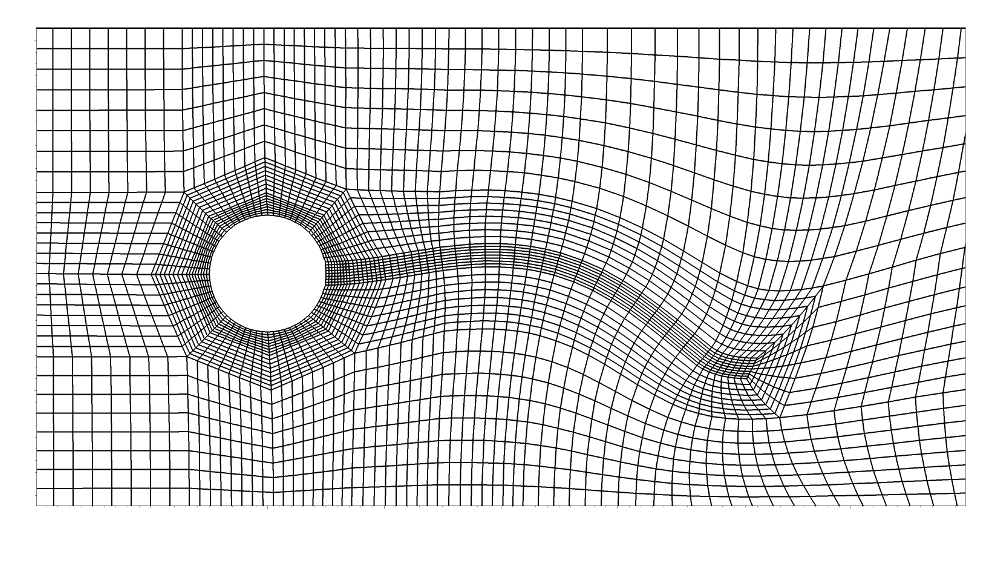
\includegraphics[width=6cm]{Pictures/visit_fsi_2_CNn_t_2e-2_global_3_biharmonic_mesh8070_scale.png}}
{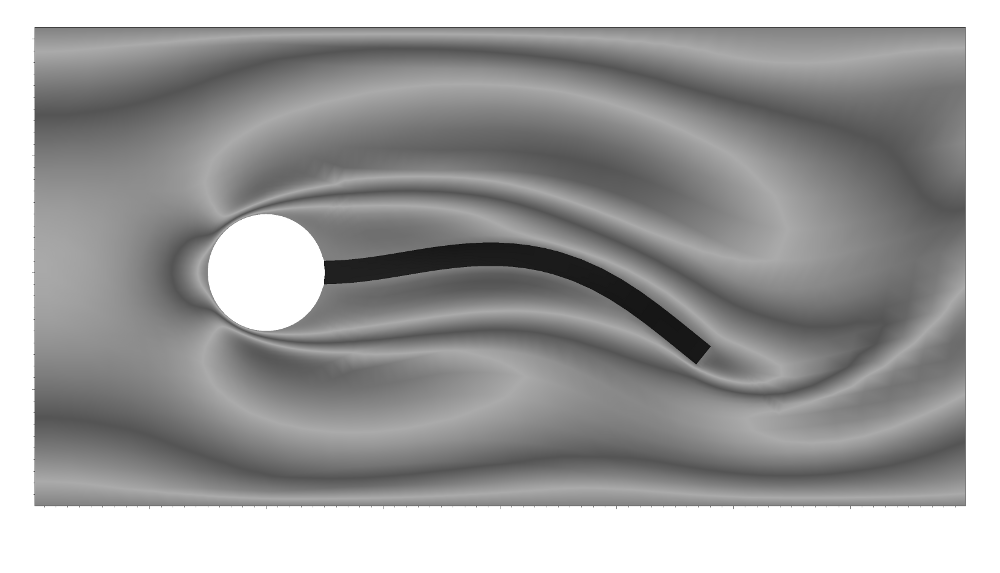
\includegraphics[width=6cm]{Pictures/visit_fsi_2_CNn_t_2e-2_global_3_biharmonic_x_velo8070_scale.png}}
\caption{FSI 2 test case: mesh (left) and velocity profile in vertical 
direction (right) at time $t=16.14s$.}
\label{res:fsi_2_mesh_and_x_velo}
\end{figure}

\begin{figure}
\centering
{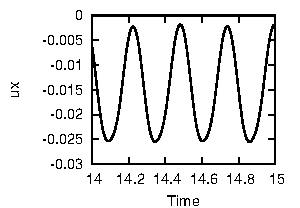
\includegraphics[width=5.8cm]{Pictures/ux_FSI_2_FS_t_3e-2_t_15e-3_global_2_Hron_grid.pdf}}
{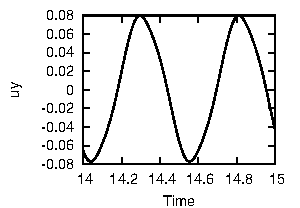
\includegraphics[width=5.8cm]{Pictures/uy_FSI_2_FS_t_3e-2_t_15e-3_global_2_Hron_grid.pdf}}
{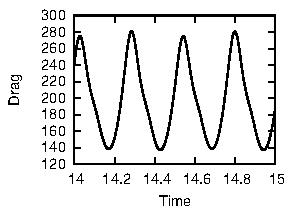
\includegraphics[width=5.8cm]{Pictures/Drag_fluid_FSI_2_FS_t_3e-2_t_15e-3_global_2_Hron_grid.pdf}}
{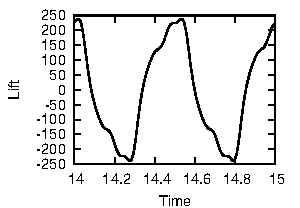
\includegraphics[width=5.8cm]{Pictures/Lift_fluid_FSI_2_FS_t_3e-2_t_15e-3_global_2_Hron_grid.pdf}}
\caption{FSI 2: the deflections of the beam, $u_x(A)$ and $u_y(A)$ (in $cm$), and 
the drag and the lift evaluation (in $kg/m\,s^2$) are displayed versus
time (in $s$).
} 
\label{res:results_ux_and_uy_fsi_2}
\end{figure}


\subsection{Compliance minimization}
Winni
Results already obtained.






%%%%%%%%%%%%%%%%%%%%%%%%%%%%%%%%%%%%%%%%%%%
\section{Conclusions}
\label{conclusions}
In this article, we described the features 
and applications of the DOpElib project, which 
was initiated at the Heidelberg University in 2010.
Specifically, the applications cover a broad 
spectrum of numerical exmamples motivated 
by different disciplines. 
Currently, we are developing concepts for the efficient 
numerical solution of time-dependent optimization
problems governed by PDEs. 

\section{Outlook}
\todo{Was wollen wir noch in den nächsten 1-2 Jahren erreichen?}

%%%%%%%%%%%%%%%%%%%%%%%%%%%%%%%%%%%%%%%%%%%
%\bibliographystyle{abbrvnat}
\bibliographystyle{acmsmall}
\bibliography{lit}
%


\end{document}


